\documentclass[aspectratio=169]{beamer}
\setbeamerfont{headline}{size=\footnotesize}

\mode<presentation>{
    \usetheme{Montpellier}
    \setbeamercovered{transparent}
    \usecolortheme{beaver}
}

\usepackage[english,brazil]{babel}
\usepackage[utf8]{inputenc}
\usepackage{fontawesome5}
\usepackage{graphicx}
\usepackage{url}
\usepackage{colortbl}
\usepackage{caption}
\usepackage{booktabs}
\usepackage{tikz}
\usetikzlibrary{positioning,arrows.meta,fit,backgrounds,shapes.multipart,
                shapes,arrows,calc,trees}
\usepackage{pgfplots}
\pgfplotsset{compat=1.18}
\usepackage{ragged2e}

% Cores
\definecolor{mineblue}{RGB}{0,90,180}
\definecolor{mineorange}{RGB}{230,115,0}
\definecolor{minegreen}{RGB}{34,139,34}
\definecolor{minered}{RGB}{180,20,40}
\definecolor{minegray}{RGB}{100,100,100}

% Comandos auxiliares
\newcommand{\reflexao}[1]{\begin{alertblock}{Reflexão}#1\end{alertblock}}
\newcommand{\key}[1]{\underline{#1}}
\newcommand{\citacao}[1]{\hfill\textcolor{minegray}{\tiny #1}}

% Dados do título
\title[Mineração de Dados]{Mineração de Dados: Conceitos e Aplicações}
\subtitle{Módulo 7: Aplicações}
\author[Elton Sarmanho]{
    Prof. Elton Sarmanho\inst{1}\\
    \footnotesize \href{mailto:eltonss@ufpa.br}{eltonss@ufpa.br}
}
\institute[UFPA]{
    \inst{1} Faculdade de Sistemas de Informação - UFPA Campus Cametá
}
\date{\today}

% Estilos TikZ
\tikzstyle{block} = [rectangle,draw,fill=mineblue!20,text width=5em,
                     text centered,rounded corners,minimum height=3em,
                     font=\small]
\tikzstyle{line}  = [draw,-latex']

\begin{document}

% ==============================================================================
% Título
% ==============================================================================
\begin{frame}
    \titlepage
    \begin{center}
        \tiny \faIcon{github}\ \href{https://github.com/eltonsarmanho}{github.com/eltonsarmanho} \quad
        \faIcon{linkedin}\ \href{https://www.linkedin.com/in/elton-sarmanho-836553185/}{Elton Sarmanho}
    \end{center}
\end{frame}

% Roteiro
\begin{frame}{Roteiro da Aula}
    \tableofcontents[sections={1-3}]
\end{frame}

\begin{frame}{Roteiro da Aula}
   \tableofcontents[sections={4-9}]
\end{frame}

% ==============================================================================
\section{Por que RAG?}
% ==============================================================================

\subsection{Limitações dos LLMs}

\begin{frame}[shrink=5]{Limitações dos LLMs ``Puros''}
    \begin{columns}
        \column{0.55\textwidth}
        \begin{alertblock}{Problemas}
            \begin{itemize}\footnotesize
                \item \textbf{Alucinação:} gera texto plausível, porém factualmente incorreto
                \item \textbf{Conhecimento desatualizado:} \textit{knowledge cutoff} do treinamento
                \item \textbf{Sem dados privados:} não conhece documentos internos, currículos, artigos específicos
                \item \textbf{Falta de rastreabilidade:} não cita fontes verificáveis
            \end{itemize}
        \end{alertblock}
        \column{0.45\textwidth}
        \pause
        \begin{block}{Analogia}
            \footnotesize Um LLM ``puro'' é um estudante fazendo prova \textbf{de memória}.\\[4pt]
            Um sistema RAG é um estudante fazendo prova \textbf{de consulta}: busca nas anotações antes de responder.
        \end{block}
    \end{columns}
\end{frame}

\begin{frame}{RAG como consulta a evidências}
    \centering
    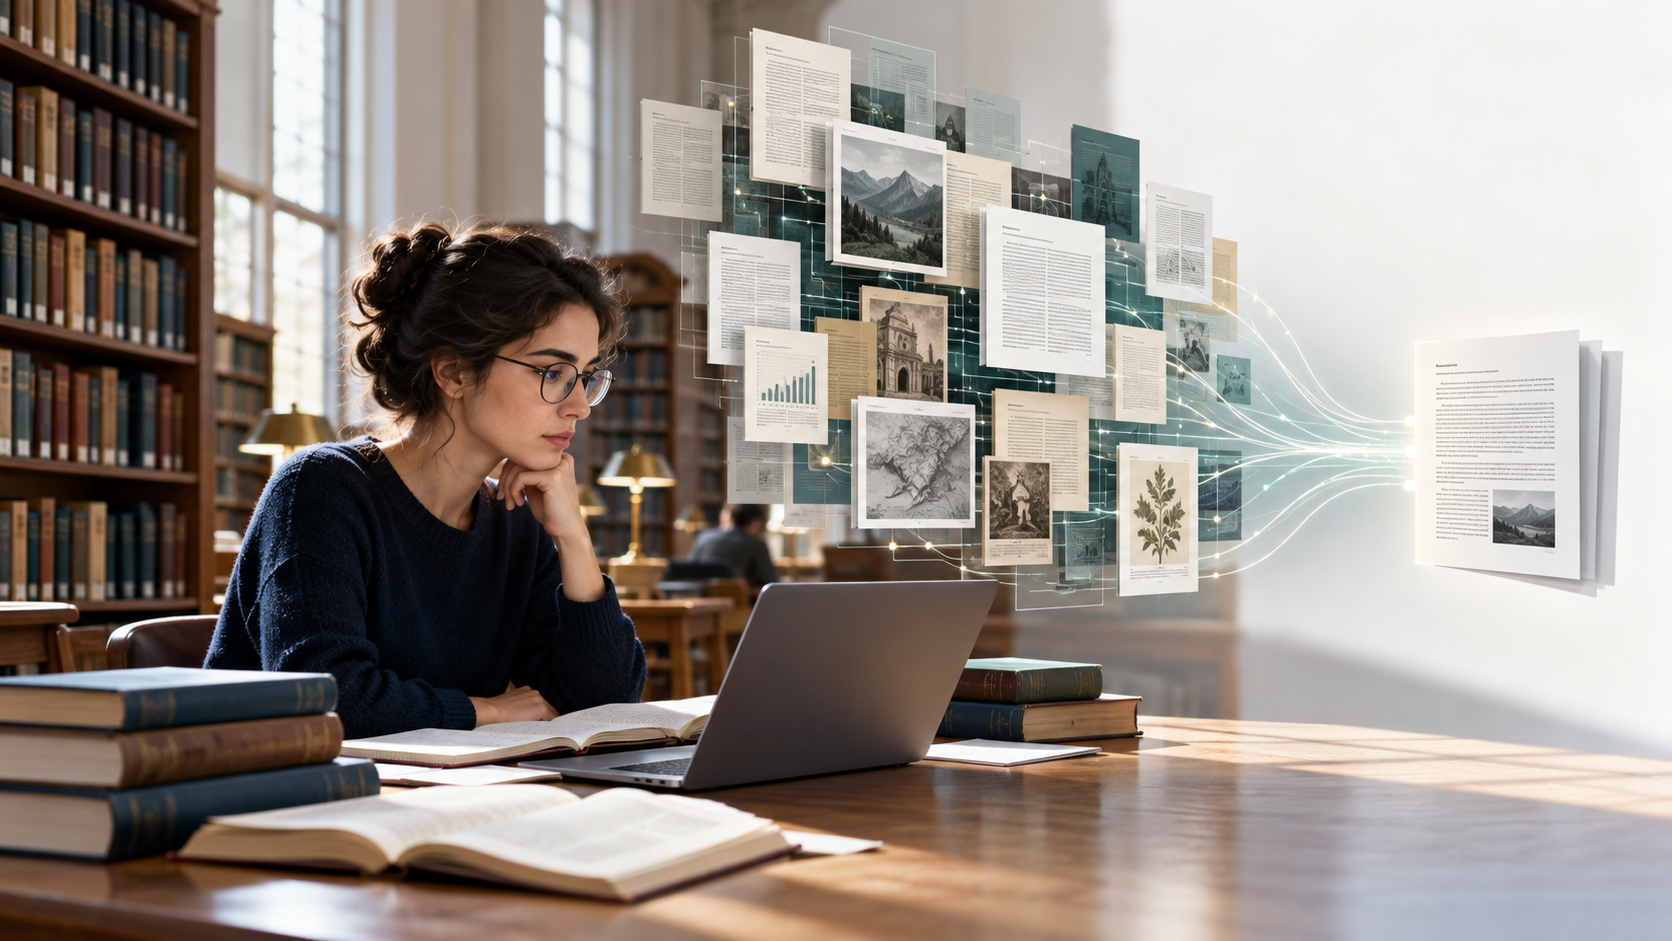
\includegraphics[width=0.6\textwidth,height=0.40\textheight,keepaspectratio]{img/rag_consulta_acervo.png}
    \captionof{figure}{Um \textit{agent} consulta documentos do acervo antes de formular uma resposta.}
    \reflexao{Qual informação da fonte precisa acompanhar a resposta para que o estudante possa conferi-la?}
\end{frame}

\begin{frame}{Retrieval-Augmented Generation (RAG)}
    \begin{block}{Definição (Lewis et al., 2020)}
        \footnotesize
        Arquitetura que combina um mecanismo de \textbf{recuperação de informação} sobre uma base externa com um modelo de \textbf{geração de linguagem}, condicionando a resposta a evidências recuperadas dinamicamente.
    \end{block}
    \pause
    \[
      p(y \mid x) \approx \sum_{z \in \mathcal{Z}_k(x)} p_{\eta}(z \mid x)\; p_{\theta}(y \mid x, z)
    \]
    \footnotesize $\mathcal{Z}_k(x)$: $k$ evidências recuperadas para a pergunta $x$; $p_\eta$: \textit{retriever}; $p_\theta$: gerador; $z$: evidência.
    \pause
    \begin{alertblock}{}
        \footnotesize RAG e \textit{fine-tuning} resolvem problemas diferentes. RAG atualiza conhecimento e permite atribuição de fontes; \textit{fine-tuning} altera comportamento ou adapta o modelo a uma tarefa.
    \end{alertblock}
\end{frame}

\subsection{Arquitetura e Paradigmas}

\begin{frame}{Pipeline RAG: Visão Geral}
    \centering
    \begin{tikzpicture}[
      box/.style={rectangle,draw=mineblue,fill=mineblue!8,rounded corners,
      minimum width=2.05cm,minimum height=.78cm,align=center,font=\footnotesize},
      arrow/.style={-{Stealth[length=5pt]},mineblue,thick}
    ]
      \node[box] (docs) {Documentos\\+ metadados};
      \node[box,right=.55cm of docs] (chunks) {Divisão em\\fragmentos};
      \node[box,right=.55cm of chunks] (index) {\textit{Embeddings}\\[-1pt] e índice};
      \node[box,right=.55cm of index] (store) {Banco\\vetorial};
      \draw[arrow] (docs)--(chunks); \draw[arrow] (chunks)--(index); \draw[arrow] (index)--(store);
      \node[box,fill=minegreen!12,draw=minegreen,below=1.25cm of store] (retrieve) {Pergunta $\to$\\recuperação};
      \node[box,fill=minered!12,draw=minered,left=.7cm of retrieve] (llm) {LLM com\\evidências};
      \node[box,fill=mineorange!12,draw=mineorange,left=.7cm of llm] (answer) {Resposta com\\citações};
      \draw[arrow] (store)--(retrieve); \draw[arrow] (retrieve)--(llm); \draw[arrow] (llm)--(answer);
    \end{tikzpicture}
    \reflexao{Em que etapa uma referência de página ou seção deve acompanhar o fragmento para que a resposta possa ser auditada?}
\end{frame}

\begin{frame}[shrink=5]{Pipeline RAG: Diagrama Esquemático}
    \centering
    \begin{tikzpicture}[
      box/.style={rectangle,draw=mineblue,fill=mineblue!8,rounded corners,
                  minimum width=2.3cm,minimum height=1.0cm,align=center,font=\small},
      arr/.style={-{Stealth[length=6pt]},mineblue,thick}
    ]
      \node[box] (doc)  at (0,0)    {\faIcon{file-alt}\\ Documentos};
      \node[box] (split) at (2.9,0) {\faIcon{cut}\\ Chunks};
      \node[box] (emb)  at (5.8,0)  {\faIcon{database}\\ Embeddings};
      \node[box,fill=mineorange!12,draw=mineorange] (vec) at (8.7,0) {\faIcon{server}\\ Banco Vetorial};
      \node[box,fill=minegreen!12,draw=minegreen] (ret) at (8.7,-2.0) {\faIcon{search}\\ Busca Semântica};
      \node[box,fill=minered!12,draw=minered] (llm) at (5.8,-2.0)  {\faIcon{robot}\\ LLM Gerador};
      \node[box] (ans) at (2.9,-2.0) {\faIcon{comment}\\ Resposta};
      \node[box,dashed] (query) at (0,-2.0) {\faIcon{question}\\ Pergunta};
      \draw[arr] (doc) -- (split);
      \draw[arr] (split) -- (emb);
      \draw[arr] (emb) -- (vec);
      \draw[arr] (vec) -- (ret);
      \draw[arr] (query.south) -- ++(0,-0.70) -| (ret.south);
      \draw[arr] (ret) -- (llm);
      \draw[arr] (llm) -- (ans);
    \end{tikzpicture}
\end{frame}

\begin{frame}{Paradigmas de RAG (Gao et al., 2024)}
    \begin{block}{Naive RAG}
        \footnotesize Pipeline direto: indexar $\to$ recuperar $\to$ gerar. É um bom ponto de partida, mas pode trazer contexto redundante ou insuficiente.
    \end{block}
    \pause
    \begin{block}{Advanced RAG}
        \footnotesize Adiciona reescrita de consultas, \textit{re-ranking} e compressão de contexto antes/depois da recuperação.
    \end{block}
    \pause
    \begin{block}{Modular RAG}
        \footnotesize Arquitetura flexível com módulos intercambiáveis: roteamento, memória, busca híbrida, iteração múltipla.
    \end{block}
\end{frame}

% ==============================================================================
\section{Divisão dos Dados}
% ==============================================================================

\subsection{Carregamento de Documentos}

\begin{frame}{Document Loading: Carregamento de Documentos}
    \begin{columns}
        \column{0.5\textwidth}
        \begin{block}{Dados Estruturados}
            \footnotesize Tabelas, planilhas, bancos relacionais e CSV/JSON costumam seguir um esquema definido.
        \end{block}
        \column{0.5\textwidth}
        \begin{block}{Dados Não Estruturados}
            \footnotesize PDFs, páginas web, áudio, vídeo e e-mails exigem extração e \textit{parsers} adequados.
        \end{block}
    \end{columns}
    \pause
    \begin{alertblock}{Importante}
        \footnotesize Preserve metadados como página, seção, autor e data. Eles permitem localizar e citar a fonte na resposta final.
    \end{alertblock}
\end{frame}

\subsection{Chunking}

\begin{frame}{Por que Dividir Documentos em \textit{Chunks}?}
    \begin{block}{Motivação}
        \footnotesize Mesmo quando cabem na janela de contexto, documentos inteiros tornam a recuperação menos seletiva. Fragmentos bem formados ligam uma evidência específica à pergunta.
    \end{block}
    \pause
    \begin{exampleblock}{Divisão Mal Feita}
        \footnotesize \textit{``O novo modelo da Renault é o Duster, possui 110 cavalos...''} dividido ingenuamente em:
        \begin{itemize}\footnotesize
            \item \texttt{"O novo modelo da Renault é"}
            \item \texttt{"o Duster, possui 110"}
            \item \texttt{"cavalos de potência..."}
        \end{itemize}
        Nenhum fragmento isolado responde ``Qual o preço do Duster?''
    \end{exampleblock}
\end{frame}

\begin{frame}{\texttt{chunk\_size} e \texttt{chunk\_overlap}}
    \begin{columns}
        \column{0.55\textwidth}
        \centering
        \begin{tikzpicture}[font=\scriptsize]
          \draw[fill=mineblue!16,draw=mineblue] (0,1.25) rectangle (3.8,1.78);
          \draw[fill=minegreen!18,draw=minegreen] (1.20,.60) rectangle (5.00,1.13);
          \draw[fill=mineorange!22,draw=mineorange] (2.40,-.05) rectangle (6.20,.48);
          \node at (1.9,1.515) {fragmento 1};
          \node at (3.1,.865) {fragmento 2};
          \node at (4.3,.215) {fragmento 3};
          \draw[<->,thick] (1.20,2.08) -- node[above]{\textit{overlap}} (3.80,2.08);
          \draw[densely dashed,gray] (1.20,1.78)--(1.20,.60);
          \draw[densely dashed,gray] (3.80,1.78)--(3.80,.60);
        \end{tikzpicture}
        \column{0.45\textwidth}
        \begin{itemize}\footnotesize
            \item \textbf{chunk\_size:} tamanho do fragmento (caracteres/\textit{tokens})
            \item \textbf{chunk\_overlap:} sobreposição entre fragmentos consecutivos, evita cortar informação na fronteira
        \end{itemize}
        \pause
        \begin{alertblock}{}
            \footnotesize Fragmentos muito curtos perdem relações locais. Fragmentos muito longos aumentam ruído e custo. Ajuste com consultas reais do acervo.
        \end{alertblock}
    \end{columns}
\end{frame}

\begin{frame}[shrink=5]{Estratégias de Divisão de Texto}
    \begin{center}\footnotesize
    \begin{tabular}{>{\bfseries}p{2.6cm}p{5.8cm}p{2.6cm}}
    \toprule
    Estratégia & Funcionamento & Uso \\
    \midrule
    Fixed-size & Corta a cada $N$ unidades, com pouca noção de estrutura & Linhas ou registros uniformes \\
    Recursivo & Tenta preservar parágrafos e frases antes de cortar & Ponto de partida para prosa \\
    Estrutural & Usa sintaxe do formato (Markdown/HTML/código) & Doc.\ técnica, código \\
    Semântico & Agrupa sentenças por similaridade de \textit{embedding} & Textos longos e heterogêneos \\
    \bottomrule
    \end{tabular}
    \end{center}
    \pause
    \begin{alertblock}{Boas Práticas}
        \footnotesize Meça o tamanho em \textit{tokens} do modelo escolhido. Comece com fragmentos que preservem uma ideia completa e teste tamanho, sobreposição e $k$ com perguntas representativas. Mantenha metadados por fragmento.
    \end{alertblock}
\end{frame}

% ==============================================================================
\section{Embeddings}
% ==============================================================================

\subsection{Representação Vetorial Semântica}

\begin{frame}{O que é um Embedding?}
    \begin{block}{Definição}
        \footnotesize Representação vetorial densa $\mathbf{v} \in \mathbb{R}^d$ de um texto, onde proximidade \textbf{geométrica} reflete proximidade \textbf{semântica}.
    \end{block}
    \pause
    \begin{exampleblock}{Exemplo}
        \footnotesize ``desistência de estudantes'' e ``evasão escolar'' $\to$ vetores próximos, mesmo sem palavras em comum.
    \end{exampleblock}
    \pause
    \begin{alertblock}{Por que importa para RAG?}
        \footnotesize Permite superar a busca por palavra-chave: recupera por \textbf{significado}, não por correspondência literal.
    \end{alertblock}
\end{frame}

\begin{frame}[shrink=5]{Evolução: de TF-IDF a Embeddings Contextuais}
    \begin{center}\footnotesize
    \begin{tabular}{>{\bfseries}p{3.2cm}p{7.6cm}}
    \toprule
    Geração & Características \\
    \midrule
    TF-IDF & Vetores esparsos por frequência; sem sinônimos \\
    Word2Vec/GloVe (2013--14) & Vetores densos estáticos por palavra \\
    BERT (2018) & Vetores contextuais (dependem da frase) \\
    Modelos de sentença (2019+) & Um vetor por frase/parágrafo, otimizado para similaridade \\
    \bottomrule
    \end{tabular}
    \end{center}
\end{frame}

\begin{frame}{Similaridade de Cosseno}
    \begin{block}{Fórmula}
        \[
          \text{sim}_{\cos}(\mathbf{u}, \mathbf{v}) = \frac{\mathbf{u} \cdot \mathbf{v}}{\|\mathbf{u}\|\,\|\mathbf{v}\|} \in [-1, 1]
        \]
    \end{block}
    \pause
    \begin{alertblock}{Vetores normalizados}
        \footnotesize Quando $\|\mathbf{u}\|=\|\mathbf{v}\|=1$, a similaridade de cosseno é o produto escalar $\mathbf{u}\cdot\mathbf{v}$. Essa propriedade simplifica muitos índices vetoriais.
    \end{alertblock}
    \pause
    \begin{exampleblock}{}
        \footnotesize $\text{sim}(\text{``gosto de cachorros''}, \text{``gosto de animais''}) \gg \text{sim}(\text{``gosto de cachorros''}, \text{``tempo está ruim''})$
    \end{exampleblock}
\end{frame}

\subsection{Modelos de Embedding}

\begin{frame}{Modelos de Embedding Disponíveis}
    \begin{center}\footnotesize
    \begin{tabular}{>{\bfseries}p{3.0cm}p{2.6cm}p{5.2cm}}
    \toprule
    Modelo & Provedor & Observação \\
    \midrule
    text-embedding-3-large & OpenAI & Alta precisão, dimensão configurável, pago \\
    Modelos multimodais & Diversos & Podem representar mais de um tipo de dado, conforme o modelo e a API \\
    BGE-M3 / Jina & BAAI / Jina AI & Abertos, executáveis localmente \\
    E5 / GTE & Microsoft / Alibaba & \textit{Baseline} amplamente usado \\
    \bottomrule
    \end{tabular}
    \end{center}
    \pause
    \begin{alertblock}{MTEB: Massive Text Embedding Benchmark}
        \footnotesize Um dos principais \textit{benchmarks} públicos para comparar modelos de \textit{embedding}. Use resultados compatíveis com idioma, domínio e tipo de consulta. \faIcon{exclamation-triangle}\ Use o mesmo modelo para indexar e consultar.
    \end{alertblock}
\end{frame}

% ==============================================================================
\section{Banco de Dados Vetorial}
% ==============================================================================

\begin{frame}{Banco de Dados Vetorial (Vector Store)}
    \begin{block}{Definição}
        \footnotesize Sistema especializado em indexar e consultar eficientemente grandes coleções de vetores, retornando os $k$ mais próximos (k-NN) de uma consulta.
    \end{block}
    \pause
    \begin{alertblock}{O Problema da Escala}
        \footnotesize Busca exata k-NN custa $O(n \cdot d)$ por consulta. Em coleções grandes, índices \textbf{ANN} (\textit{Approximate Nearest Neighbors}) negociam uma pequena perda de \textit{recall} por menor latência.
    \end{alertblock}
    \pause
    \begin{itemize}\footnotesize
        \item \textbf{HNSW:} grafo hierárquico de vizinhança (Malkov \& Yashunin, 2018), com boa latência e maior uso de memória
        \item \textbf{IVF:} particiona o espaço em \textit{clusters} (K-Means)
        \item \textbf{PQ:} comprime vetores, reduz uso de memória
    \end{itemize}
\end{frame}

\begin{frame}[shrink=5]{Comparação de Soluções}
    \begin{center}\footnotesize
    \begin{tabular}{>{\bfseries}p{2.0cm}p{3.0cm}p{2.8cm}p{3.4cm}}
    \toprule
    Solução & Escala Ideal & Persistência & Observação \\
    \midrule
    Chroma & Protótipos e aplicações locais & Disponível & API simples para experimentar \\
    FAISS & Índices embarcados & A cargo da aplicação & Biblioteca rápida para busca vetorial \\
    Pinecone, Weaviate, Milvus & Serviços ou clusters & Depende da implantação & Recursos operacionais e de escalabilidade variam \\
    pgvector & Integra c/ dados relacionais & Nativa PostgreSQL & Combina busca vetorial + SQL \\
    \bottomrule
    \end{tabular}
    \end{center}
    \pause
    \begin{alertblock}{Recomendação}
        \footnotesize Escolha pelo volume, filtros por metadados, latência, custo e requisitos de operação. Compare com dados e consultas semelhantes aos do projeto.
    \end{alertblock}
\end{frame}

% ==============================================================================
\section{Busca Semântica e Recuperação}
% ==============================================================================

\subsection{Semantic Search e MMR}

\begin{frame}{Busca Semântica (\textit{Semantic Search})}
    \begin{block}{Definição}
        \footnotesize Recupera os $k$ documentos com maior similaridade de cosseno ao \textit{embedding} da consulta, por \textbf{significado}, não apenas por palavra-chave.
    \end{block}
    \pause
    \begin{columns}
        \column{0.5\textwidth}
        \begin{block}{Vantagens}
            \footnotesize\begin{itemize}\item Simples \item Baixo custo \item Ótima p/ perguntas factuais\end{itemize}
        \end{block}
        \column{0.5\textwidth}
        \begin{alertblock}{Limitações}
            \footnotesize\begin{itemize}\item Pode retornar documentos redundantes \item Sem garantia de diversidade\end{itemize}
        \end{alertblock}
    \end{columns}
\end{frame}

\begin{frame}[shrink=5]{MMR: Maximal Marginal Relevance}
    \begin{block}{Fórmula (Carbonell \& Goldstein, 1998)}
        \footnotesize
        \[
          \text{MMR} = \arg\max_{D_i \in R \setminus S} \Big[ \lambda \cdot \text{sim}(D_i, Q) - (1-\lambda) \cdot \max_{D_j \in S} \text{sim}(D_i, D_j) \Big]
        \]
    \end{block}
    \begin{columns}
        \column{0.5\textwidth}
        \centering
        \begin{tikzpicture}[scale=.78,font=\scriptsize]
          \draw[->,gray] (0,0)--(5.2,0) node[right]{dimensão 1};
          \draw[->,gray] (0,0)--(0,3.45) node[above]{dimensão 2};
          \coordinate (q) at (4.05,2.55);
          \coordinate (a) at (3.15,1.62);
          \coordinate (b) at (4.62,1.70);
          \coordinate (c) at (1.65,.68);
          \draw[densely dashed,mineblue] (q) circle (1.28);
          \draw[densely dotted,gray] (q)--(a);
          \draw[densely dotted,gray] (q)--(b);
          \draw[densely dotted,gray] (q)--(c);
          \fill[mineblue] (q) circle (3pt) node[above=2pt]{consulta $Q$};
          \fill[minegreen] (a) circle (3pt) node[below left=2pt]{A};
          \fill[minegreen] (b) circle (3pt) node[below right=2pt]{B};
          \fill[mineorange] (c) circle (3pt) node[above left=2pt]{C};
        \end{tikzpicture}
        \column{0.5\textwidth}
        \footnotesize A e B são relevantes, mas redundantes. C é menos próximo de $Q$, porém acrescenta diversidade.\\[4pt]
        $\lambda \to 1$: prioriza relevância.\\
        $\lambda \to 0$: prioriza diversidade.
        \pause
        \begin{alertblock}{Quando usar}
            \footnotesize Semantic Search: perguntas factuais.\\
            MMR: perguntas exploratórias, evita redundância.
        \end{alertblock}
    \end{columns}
\end{frame}

\begin{frame}{Busca Híbrida}
    \begin{block}{Densa + Esparsa}
        \footnotesize Combina recuperação por \textit{embeddings} (densa) com BM25 (esparsa e lexical). Os resultados podem ser fundidos por ranking ou reordenados por um \textit{reranker}.
    \end{block}
    \pause
    \begin{alertblock}{Quando usar}
        \footnotesize Consultas com termos técnicos exatos (siglas, códigos, nomes próprios) que a busca semântica pura pode não priorizar.
    \end{alertblock}
\end{frame}

\subsection{Combinando Contexto com o LLM}

\begin{frame}{Pipeline RetrievalQA}
    \centering
    \begin{tikzpicture}[
      node distance=.55cm,
      box/.style={rectangle,draw=mineblue,fill=mineblue!8,rounded corners,
      minimum width=2.15cm,minimum height=.8cm,align=center,font=\footnotesize},
      arrow/.style={-{Stealth[length=5pt]},mineblue,thick}
    ]
      \node[box] (q) {Pergunta};
      \node[box,right=of q] (r) {Recuperar\\$k$ fragmentos};
      \node[box,right=of r] (p) {\textit{Prompt} com\\evidências};
      \node[box,right=of p,fill=minegreen!12,draw=minegreen] (a) {Resposta +\\fontes};
      \draw[arrow] (q)--(r); \draw[arrow] (r)--(p); \draw[arrow] (p)--(a);
    \end{tikzpicture}
    \begin{block}{}
        \centering\footnotesize Pergunta $\to$ consulta ao banco vetorial $\to$ fragmentos relevantes $\to$ LLM $\to$ resposta.
    \end{block}
\end{frame}

\begin{frame}[shrink=5]{Estratégias de Combinação: Stuff, Map-Reduce, Refine}
    \begin{center}\footnotesize
    \begin{tabular}{>{\bfseries}p{2.0cm}p{6.6cm}p{2.8cm}}
    \toprule
    Estratégia & Funcionamento & Compromisso \\
    \midrule
    Stuff & Concatena todos os fragmentos em um único \textit{prompt} & Simples, limitada pela janela de contexto \\
    Map-Reduce & Resposta parcial por fragmento, depois combina & Escala, mais custo/latência \\
    Refine & Refina resposta iterativamente a cada fragmento & Mais contexto, sequencial e lenta \\
    \bottomrule
    \end{tabular}
    \end{center}
\end{frame}

\begin{frame}{Stuff vs.\ Map-Reduce: Diagramas}
    \begin{columns}
        \column{0.5\textwidth}
        \centering
        \textbf{Stuff}\\[3pt]
        \begin{tikzpicture}[scale=.7,font=\scriptsize,
          b/.style={rectangle,draw,rounded corners,minimum width=1.2cm,minimum height=.45cm,align=center},
          a/.style={-{Stealth},thick}]
          \node[b,fill=mineblue!12] (c1) at (0,1.2) {$c_1$};
          \node[b,fill=mineblue!12] (c2) at (1.4,1.2) {$c_2$};
          \node[b,fill=mineblue!12] (c3) at (2.8,1.2) {$c_3$};
          \node[b,fill=minered!12] (llm) at (1.4,0) {um \textit{prompt} + LLM};
          \node[b,fill=minegreen!12] (ans) at (1.4,-1) {resposta};
          \draw[a] (c1)--(llm); \draw[a] (c2)--(llm); \draw[a] (c3)--(llm); \draw[a] (llm)--(ans);
        \end{tikzpicture}
        \par\scriptsize Simples, limitado pelo contexto.
        \column{0.5\textwidth}
        \centering
        \textbf{Map-Reduce}\\[3pt]
        \begin{tikzpicture}[scale=.7,font=\scriptsize,
          b/.style={rectangle,draw,rounded corners,minimum width=1.05cm,minimum height=.45cm,align=center},
          a/.style={-{Stealth},thick}]
          \node[b,fill=mineblue!12] (c1) at (0,1.2) {$c_1$};
          \node[b,fill=mineblue!12] (c2) at (1.5,1.2) {$c_2$};
          \node[b,fill=mineblue!12] (c3) at (3,1.2) {$c_3$};
          \node[b,fill=mineorange!14] (m1) at (0,.2) {map};
          \node[b,fill=mineorange!14] (m2) at (1.5,.2) {map};
          \node[b,fill=mineorange!14] (m3) at (3,.2) {map};
          \node[b,fill=minered!12] (red) at (1.5,-.8) {reduzir};
          \draw[a] (c1)--(m1); \draw[a] (c2)--(m2); \draw[a] (c3)--(m3);
          \draw[a] (m1)--(red); \draw[a] (m2)--(red); \draw[a] (m3)--(red);
        \end{tikzpicture}
        \par\scriptsize Escala melhor, com mais chamadas ao modelo.
    \end{columns}
\end{frame}

% ==============================================================================
\section{Avaliação de Sistemas RAG}
% ==============================================================================

\begin{frame}[shrink=5]{RAGAS: Métricas de Avaliação}
    \begin{alertblock}{Duas Frentes de Falha}
        \footnotesize Um RAG pode falhar na \textbf{recuperação} (documentos errados) ou na \textbf{geração} (resposta mal formulada mesmo com contexto correto).
    \end{alertblock}
    \pause
    \begin{center}\footnotesize
    \begin{tabular}{>{\bfseries}p{2.8cm}p{8.2cm}}
    \toprule
    Métrica & Definição \\
    \midrule
    Context Precision & Proporção do contexto recuperado que é relevante (retriever) \\
    Context Recall & Proporção da informação necessária que foi recuperada (retriever) \\
    Faithfulness & Afirmações da resposta sustentadas pelo contexto (gerador) \\
    Answer Relevancy & O quanto a resposta aborda a pergunta (gerador) \\
    \bottomrule
    \end{tabular}
    \end{center}
    \pause
    \begin{block}{Diagnóstico}
        \footnotesize Precision/Recall baixos $\to$ ajustar \textit{chunking}/\textit{embedding}/busca. Faithfulness baixa $\to$ problema no LLM/\textit{prompt}.
    \end{block}
\end{frame}

% ==============================================================================
\section{Extração de Dados}
% ==============================================================================

\subsection{Palavras-chave e Tópicos}

\begin{frame}{Extração de Informação (IE)}
    \begin{block}{Definição}
        \footnotesize Processo de identificar e estruturar automaticamente palavras-chave, tópicos, entidades e relações em texto não estruturado. O resultado transforma um acervo em conhecimento organizado.
    \end{block}
    \pause
    \begin{alertblock}{Complementar ao RAG}
        \footnotesize Extração ajuda a \textbf{compreender} o acervo como um todo; RAG ajuda a \textbf{responder perguntas pontuais} sobre ele.
    \end{alertblock}
\end{frame}

\begin{frame}[shrink=5]{Extração de Palavras-chave (\textit{Keyword Extraction})}
    \begin{center}\footnotesize
    \begin{tabular}{>{\bfseries}p{2.2cm}p{7.0cm}p{2.4cm}}
    \toprule
    Método & Funcionamento & Característica \\
    \midrule
    TF-IDF & Frequência no doc.\ penalizada pelo corpus & \textit{Baseline} estatístico \\
    RAKE (2010) & Grafo de co-ocorrência de palavras & Rápido, sem treino \\
    YAKE (2020) & Estatísticas posicionais e de contexto & Independe de idioma/corpus \\
    KeyBERT (2020) & Similaridade de \textit{embedding} (BERT) & Relevância semântica \\
    \bottomrule
    \end{tabular}
    \end{center}
    \pause
    \begin{block}{Qual usar?}
        \footnotesize Triagem rápida: RAKE/YAKE. Relevância semântica (reaproveitando o \textit{embedding} do RAG): KeyBERT.
    \end{block}
\end{frame}

\begin{frame}{Modelagem de Tópicos (\textit{Topic Modeling})}
    \begin{block}{Definição}
        \footnotesize Descobre, de forma não supervisionada, os temas latentes de uma coleção de $N$ documentos.
    \end{block}
    \pause
    \begin{itemize}\footnotesize
        \item \textbf{LDA} (Blei et al., 2003): tópicos como distribuições sobre palavras; documentos como mistura de tópicos.
        \item \textbf{BERTopic} (Grootendorst, 2022): \textit{embeddings} + UMAP + HDBSCAN + c-TF-IDF. Pode produzir tópicos mais interpretáveis em corpora semânticos, mas precisa ser avaliado no domínio.
    \end{itemize}
    \pause
    \begin{exampleblock}{Aplicação}
        \footnotesize ``Quais subtemas aparecem nos $N$ artigos sobre evasão escolar? (fatores socioeconômicos, algoritmos preditivos, EAD, avaliação de modelos...)''
    \end{exampleblock}
\end{frame}

\subsection{Tendências e Relações}

\begin{frame}{Análise de Tendências (\textit{Trend Analysis})}
    \begin{block}{Combinando Tópicos + Metadados Temporais}
        \begin{enumerate}\footnotesize
            \item Extrair tópico dominante de cada documento
            \item Agrupar documentos por ano de publicação
            \item Calcular frequência relativa do tópico por período
            \item Plotar série temporal: tópicos emergentes vs.\ em declínio
        \end{enumerate}
    \end{block}
    \pause
    \begin{alertblock}{Atenção}
        \footnotesize Tendência relevante = frequência crescente \textbf{+} relevância sustentada, não apenas contagem pontual.
    \end{alertblock}
\end{frame}

\begin{frame}[shrink=5]{Extração de Relações e Grafos de Conhecimento}
    \begin{block}{NER e Relation Extraction (RE)}
        \footnotesize \textbf{NER:} identifica entidades como algoritmos, \textit{datasets} e métricas. \textbf{RE:} conecta pares de entidades por relações, por exemplo, \textit{Random Forest} utilizado em predição de evasão escolar.
    \end{block}
    \pause
    \begin{columns}
        \column{0.5\textwidth}
        \begin{block}{Abordagem Clássica}
            \footnotesize Pipeline NER (spaCy) + classificador de relações.
        \end{block}
        \column{0.5\textwidth}
        \begin{block}{Abordagem via LLM}
            \footnotesize Um \textit{prompt} pode retornar entidades e relações em JSON, mas a saída exige validação.
        \end{block}
    \end{columns}
    \pause
    \begin{alertblock}{}
        \footnotesize \faIcon{exclamation-triangle}\ Entidades/relações extraídas por LLM também podem ser alucinadas. Valide contra o texto de origem. O grafo resultante é o insumo do \textbf{GraphRAG}.
    \end{alertblock}
\end{frame}

% ==============================================================================
\section{Estudo de Caso: Chatbot RAG}
% ==============================================================================

\begin{frame}[shrink=5]{Chatbot RAG sobre um Acervo de Artigos Científicos}
    \centering
    \begin{tikzpicture}[
      box/.style={rectangle,draw=mineblue,fill=mineblue!8,rounded corners,
                  minimum width=2.7cm,minimum height=0.95cm,align=center,font=\footnotesize},
      arr/.style={-{Stealth[length=6pt]},mineblue,thick}
    ]
      \node[box] (pdfs) at (0,0) {\faIcon{file-pdf}\\ Artigos (PDF)};
      \node[box] (chunks) at (3.1,0) {\faIcon{cut}\\ Chunking};
      \node[box] (emb) at (6.2,0) {\faIcon{database}\\ Embeddings};
      \node[box,fill=mineorange!12,draw=mineorange] (store) at (6.2,-1.6) {\faIcon{server}\\ Chroma/FAISS};
      \node[box,fill=minegreen!12,draw=minegreen] (mmr) at (3.1,-1.6) {\faIcon{search}\\ Retriever};
      \node[box,fill=minered!12,draw=minered] (chat) at (0,-1.6) {\faIcon{comments}\\ Chatbot};
      \draw[arr] (pdfs) -- (chunks);
      \draw[arr] (chunks) -- (emb);
      \draw[arr] (emb) -- (store);
      \draw[arr] (store) -- (mmr);
      \draw[arr] (mmr) -- (chat);
    \end{tikzpicture}
    \pause
    \begin{block}{Etapas (implementadas no Colab)}
        \footnotesize 1. Carregamento $\to$ 2. Extração exploratória (palavras-chave/tópicos) $\to$ 3. Chunking $\to$ 4. Embedding + Indexação $\to$ 5. Retriever (semântico/MMR) $\to$ 6. RetrievalQA $\to$ 7. Interface conversacional $\to$ 8. Avaliação (RAGAS)
    \end{block}
\end{frame}

\begin{frame}{Limitações a Considerar no Projeto}
    \begin{alertblock}{}
        \begin{itemize}\footnotesize
            \item O chatbot só responde bem sobre o que está no acervo indexado
            \item Perguntas multi-documento podem exigir Map-Reduce ou GraphRAG
            \item \texttt{chunk\_size} e $k$ do \textit{retriever} são hiperparâmetros a ajustar empiricamente
        \end{itemize}
    \end{alertblock}
    \vspace{0.3cm}
    \centering\footnotesize \faIcon{arrow-right}\ Implementação completa e código no notebook Colab deste módulo.
\end{frame}

% ==============================================================================
\section{Qualidade, Segurança e Tendências}

\begin{frame}{Segurança e Governança em RAG}
    \begin{columns}
      \column{.5\textwidth}
      \begin{alertblock}{Riscos}
        \footnotesize
        \begin{itemize}
          \item Documento malicioso pode tentar alterar instruções do LLM
          \item Recuperar um trecho não autoriza expor dados pessoais ou sigilosos
          \item Citação aumenta auditabilidade, mas não prova que a conclusão está correta
        \end{itemize}
      \end{alertblock}
      \column{.5\textwidth}
      \begin{block}{Controles}
        \footnotesize
        \begin{itemize}
          \item Controle de acesso antes da recuperação
          \item Separar instruções do sistema, consulta e documentos
          \item Registrar fontes e avaliar respostas antes da implantação
        \end{itemize}
      \end{block}
    \end{columns}
    \reflexao{Se um estudante só pode ler parte do acervo, em qual etapa essa permissão deve ser aplicada?}
\end{frame}

\begin{frame}{Acesso responsável ao acervo}
    \centering
    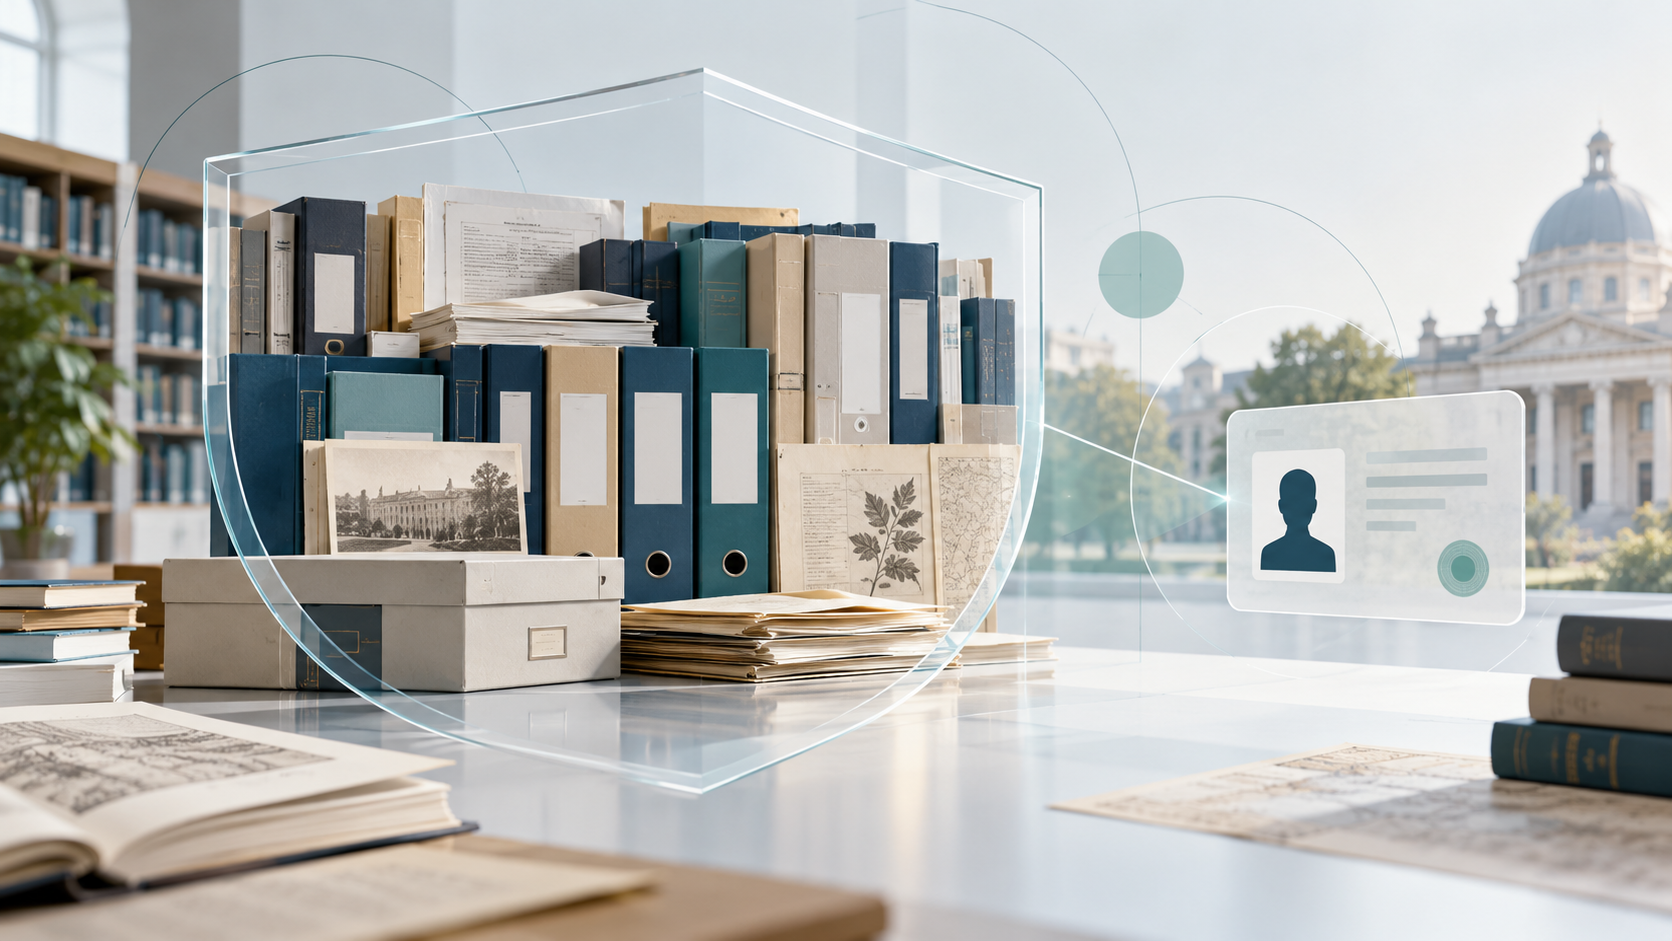
\includegraphics[width=0.6\textwidth,height=0.40\textheight,keepaspectratio]{img/rag_acesso_controlado.png}
    \captionof{figure}{Em um sistema RAG, a recuperação deve respeitar as permissões de acesso ao acervo.}
    \reflexao{Por que é insuficiente verificar a permissão do usuário apenas depois que o documento já foi recuperado?}
\end{frame}

\subsection{Tendências de Pesquisa}
% ==============================================================================

\begin{frame}[shrink=5]{Estado da Arte: Self-RAG e Corrective RAG}
    \begin{block}{Self-RAG (Asai et al., 2023)}
        \footnotesize Treina o modelo para emitir \textit{tokens} de reflexão que decidem quando recuperar, se os documentos são relevantes e se a resposta é sustentada pelo contexto.
    \end{block}
    \pause
    \begin{block}{Corrective RAG (CRAG, Yan et al., 2024)}
        \footnotesize Um avaliador classifica a qualidade dos documentos recuperados e pode disparar recuperação complementar quando a confiança é baixa.
    \end{block}
\end{frame}

\begin{frame}{Estado da Arte: GraphRAG e RAG Agêntico}
    \begin{block}{GraphRAG (Microsoft Research, 2024)}
        \footnotesize Constrói um grafo de entidades a partir dos documentos e pode sumarizar comunidades. É útil para perguntas globais ou com múltiplos saltos, desde que a extração do grafo seja confiável.
    \end{block}
    \pause
    \begin{block}{RAG Agêntico (\textit{Agentic RAG})}
        \footnotesize Um agente decide quantas recuperações executar, quais ferramentas consultar e quando encerrar. A flexibilidade vem acompanhada de mais custo, latência e necessidade de avaliação.
    \end{block}
    \vspace{0.2cm}
    \centering\tiny \faIcon{arrow-right}\ Material Didático e Colab trazem o pipeline completo do chatbot RAG
\end{frame}

% ==============================================================================
% Referências
% ==============================================================================
\begin{frame}[shrink=11]{Referências Bibliográficas}
    \begin{thebibliography}{99}\footnotesize
        \bibitem{lewis} Lewis, P. et al. \textit{Retrieval-Augmented Generation for Knowledge-Intensive NLP Tasks}. NeurIPS, 2020.
        \bibitem{gao} Gao, Y. et al. \textit{Retrieval-Augmented Generation for Large Language Models: A Survey}. arXiv:2312.10997, 2024.
        \bibitem{asai} Asai, A. et al. \textit{Self-RAG: Learning to Retrieve, Generate, and Critique through Self-Reflection}. arXiv:2310.11511, 2023.
        \bibitem{yan} Yan, S.-Q. et al. \textit{Corrective Retrieval Augmented Generation}. arXiv:2401.15884, 2024.
        \bibitem{edge} Edge, D. et al. \textit{From Local to Global: A Graph RAG Approach}. Microsoft Research, arXiv:2404.16130, 2024.
        \bibitem{carbonell} Carbonell, J.; Goldstein, J. \textit{The Use of MMR, Diversity-Based Reranking}. SIGIR, 1998.
        \bibitem{blei} Blei, D. M. et al. \textit{Latent Dirichlet Allocation}. JMLR, 2003.
        \bibitem{grootendorst} Grootendorst, M. \textit{BERTopic: Neural Topic Modeling with a Class-based TF-IDF Procedure}. arXiv:2203.05794, 2022.
        \bibitem{material} \textbf{Material Didático Módulo 7} e Notebook Colab disponíveis no repositório da disciplina.
    \end{thebibliography}
\end{frame}

\end{document}
